\subsection{Modellazione dei casi d'uso}

\subsubsection{Attori e casi d'uso}

\begin{flushleft}

\textbf{\textit{\underline{Attori primari}}}:

\begin{itemize}
    \item {Utente}
    \item {Utente registrato}
    \item {Gestore dell'applicazione}
\end{itemize}

\textbf{\textit{\underline{Casi d'uso}}}:

\begin{itemize}
    \item {UC1: Registrazione}
    \item {UC2: CondividiViaggio}
    \item {UC3: RicercaViaggio}
    \item {UC4: Login}
    \item {UC5: ValutaUtente}
    \item {UC6: VisualizzaPrenotazioni}
    \item {UC7: GeneraReportIncassi}
    \item {UC8: GeneraReportUtenti}
    \item {UC9: AggiornaDatiPersonali}
\end{itemize}

\textbf{\textit{\underline{Casi d'uso di inclusione}}}:
\begin{itemize}
    \item {UC10: GestisciPrenotazione}
\end{itemize}


\textbf{\textit{\underline{Casi d'uso di estensione}}}:
\begin{itemize}
    \item {UC11: PrenotaViaggio}
\end{itemize}


\begin{tabularx}{\textwidth}{|0{p{4.5cm}}|0{p{2.7cm}}|0{p{4.3cm}}|0{X}|}
\hline
\textbf{Caso d'uso} & \textbf{Attori Primari} & \textbf{Incl./Ext.} & \textbf{Requisiti corrispondenti} \\ \hline
UC1: Registrazione & Utente & - & $RF_1$ \\ \hline
UC2: CondividiViaggio & Utente registrato & - & $RF_2$ \\ \hline
UC3: RicercaViaggio & Utente registrato & - & $RF_3$ \\ \hline
UC4: Login & Utente registrato & - & $RF_{10}$ \\ \hline
UC5: ValutaUtente & Utente registrato & - & $RF_8$ \\ \hline
UC6: VisualizzaPrenotazioni & Utente registrato & Incluso in GestisciPrenotazione & $RF_5$ \\ \hline
UC7: GeneraReportIncassi & Gestore dell'applicazione & - & $RF_9$ \\ \hline
UC8: GeneraReportUtenti & Gestore dell'applicazione & - & $RF_9$ \\ \hline
UC9: AggiornaDatiPersonali & Utente registrato & - & $RF_{11}$ \\ \hline
UC10: GestisciPrenotazione & Utente registrato & Include VisualizzaPrenotazioni & $RF_{6\mbox{,}7}$ \\ \hline
UC11: PrenotaViaggio & - & Estensione di RicercaViaggio & $RF_4$ \\ \hline
\end{tabularx}

\end{flushleft}

\subsubsection{Diagramma dei casi d'uso}

\begin{figure}[H]
    \centering
    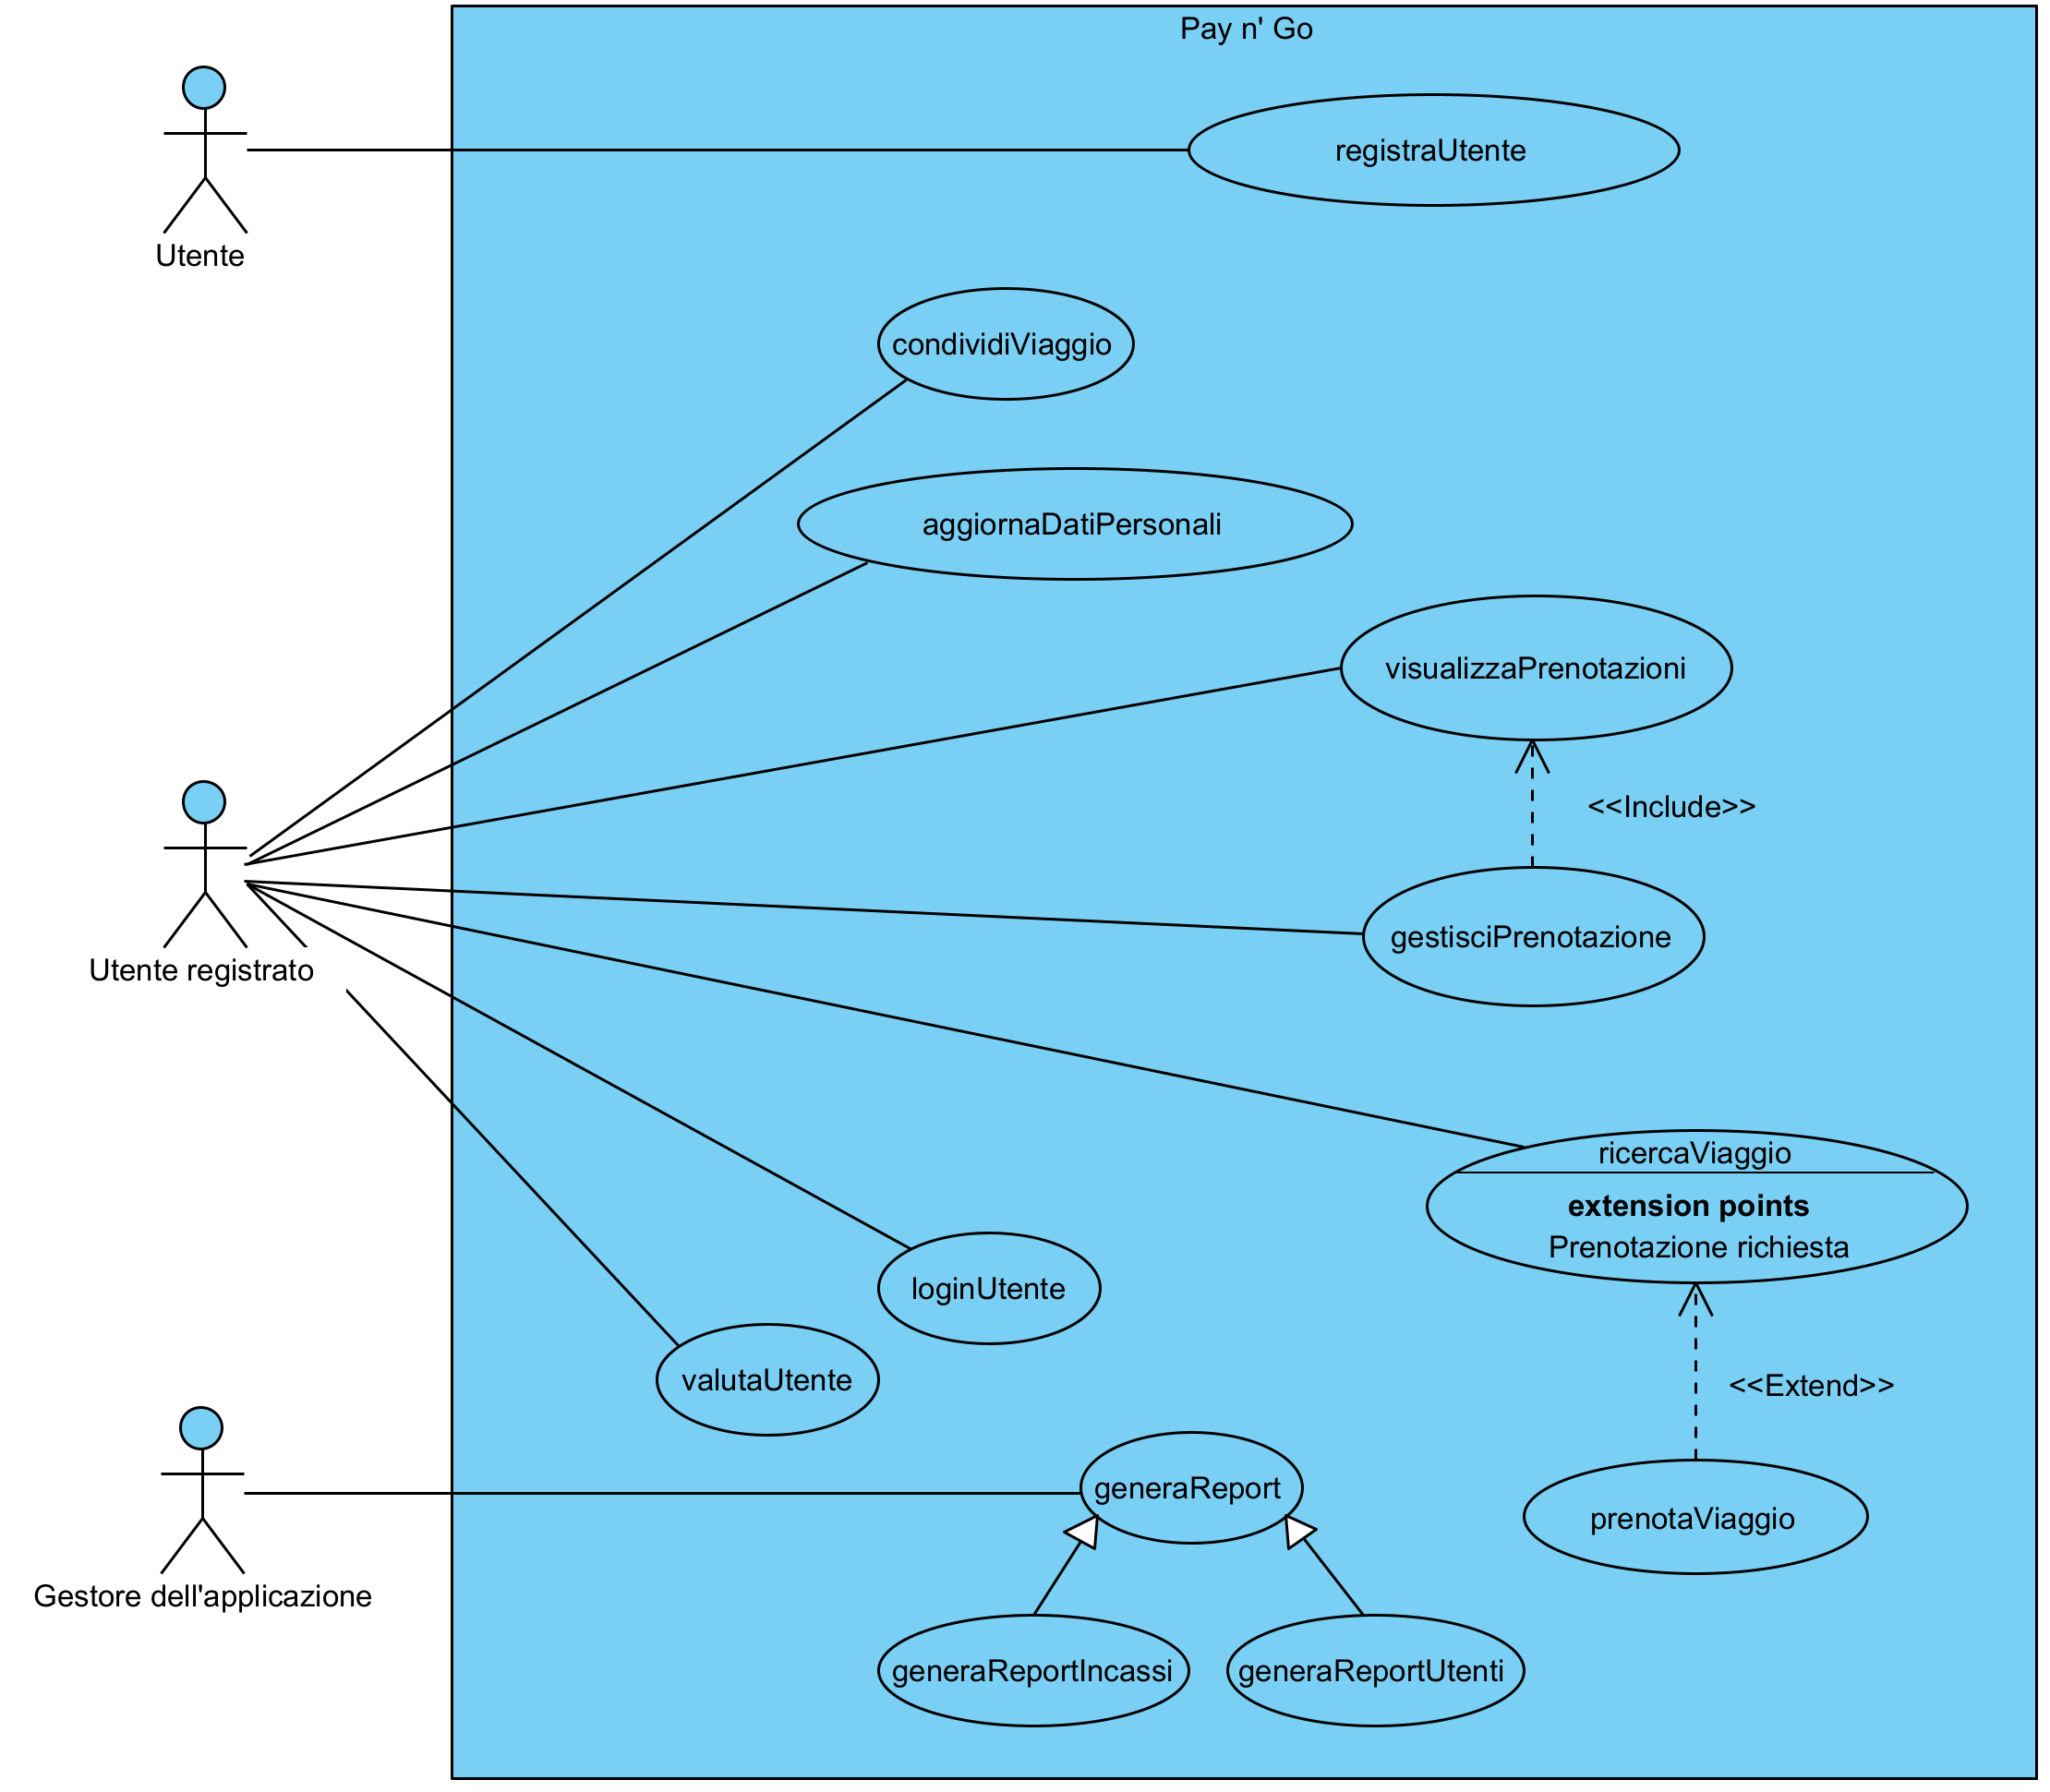
\includegraphics[scale=0.8]{img/diagrams/use_case_diagram.png}
    \caption{Diagramma dei casi d'uso}
\end{figure}

\subsubsection{Scenari}

\begin{flushleft}
\begin{usecase}
    \name{\textbf{Registrazione}}
    \actor{Utente}
    \udescription{Un Utente effettua la procedura di registrazione}
    \precondition{}
    \scenario{
        \item {Il caso d'uso ha inizio quando l'Utente richiede la registrazione al sistema}
        \item {Il sistema mostra all'Utente un'interfaccia in cui inserire i propri dati: nome, cognome, contatto telefonico, indirizzo email, password, tipo di automobile e numero di posti disponibili}
        \item {L'Utente inserisce i dati richiesti}
        \item {Il sistema controlla che l'Utente non sia già registrato}
        \begin{tabenum}
            \item {Se l'Utente è già registrato, il sistema mostra un opportuno messaggio di errore}
        \end{tabenum}
        \item {Il sistema memorizza i dati inseriti e notifica l'Utente dell'avvenuta registrazione}
    }
    \result{L'Utente è stato correttamente registrato}
    \extensions{}
    \exceptions{
        \item[3.a.]{L'Utente inserisce dati non validi}
        \begin{tabenum}
            \item[3.a.1.]{Il sistema segnala l'errore e chiede di inserire dei dati validi}
        \end{tabenum}
    }
\end{usecase}

\vspace{1cm}

\begin{usecase}
    \name{\textbf{CondividiViaggio}}
    \actor{Utente registrato}
    \udescription{Un Utente registrato condivide i dettagli di un viaggio}
    \precondition{L'Utente è stato autenticato dal sistema e ha un'automobile associata}
    \scenario{
        \item {Il caso d'uso ha inizio quando l'Utente registrato richiede al sistema di condividere i dettagli di un viaggio}
        \item {Il sistema mostra all'Utente registrato un'interfaccia in cui inserire le informazioni circa il viaggio: luogo di partenza, luogo di destinazione, data ed ora di partenza e contributo per le spese di viaggio}
        \item {L'Utente inserisce i dati richiesti}
        \item {Il sistema memorizza le informazioni del viaggio condiviso e notifica all'Utente l'avvenuta condivisione}
    }
    \result{L'Utente ha condiviso correttamente un viaggio}
    \extensions{}
    \exceptions{
        \item[3.a] L’Utente inserisce dati non validi
        \begin{tabenum}
            \item[3.a.1.]{Il sistema segnala l'errore e chiede di inserire dei dati validi}
        \end{tabenum}
    }
\end{usecase}

\vspace{1cm}

\begin{usecase}
    \name{\textbf{RicercaViaggio}}
    \actor{Utente registrato}
    \udescription{Un Utente registrato effettua la ricerca di un viaggio}
    \precondition{L'Utente è stato autenticato dal sistema}
    \scenario{
        \item {Il caso d'uso ha inizio quando l'Utente registrato richiede al sistema di ricercare un viaggio}
        \item {Il sistema mostra all'Utente registrato un'interfaccia in cui inserire i criteri di ricerca: luogo di partenza, luogo di destinazione e data ed ora di partenza}
        \item {L'Utente inserisce i dati richiesti}
        \item {Se il sistema trova uno o più viaggi}
        \begin{tabenum}
            \item {Per ogni viaggio trovato}
            \begin{tabenum}
              \item {Il sistema ne mostra i dettagli}
            \end{tabenum}
        \end{tabenum}
        \item {Altrimenti}
        \begin{tabenum}
            \item {Il sistema comunica all'Utente registrato che non sono stati trovati viaggi corrispondenti ai criteri di ricerca}
        \end{tabenum}
        \item {\textbf{Punto di estensione}: prenotazione richiesta}
    }
    \result{}
    \extensions{}
    \exceptions{
        \item[3.a] L’Utente inserisce dati non validi
        \begin{tabenum}
            \item[3.a.1.]{Il sistema segnala l'errore e chiede di inserire dei dati validi}
        \end{tabenum}
    }
\end{usecase}

\vspace{1cm}

\begin{usecase}
    \name{\textbf{Login}}
    \actor{Utente registrato}
    \udescription{Un Utente registrato effettua la procedura di login}
    \precondition{L'Utente non è autenticato dal sistema}
    \scenario{
        \item {Il caso d'uso ha inizio quando l'Utente registrato richiede di effettuare il login al sistema}
        \item {Il sistema mostra all'Utente registrato un'interfaccia in cui inserire i dati per effettuare il login: indirizzo email e password}
        \item {L'Utente inserisce i dati richiesti}
        \item {Il sistema verifica la validità dei dati inseriti}
        \item {Il sistema comunica all'Utente l'avvenuta autenticazione}
    }
    \result{L'Utente viene correttamente autenticato dal sistema}
    \extensions{
        
    }
    \exceptions{
        \item[4.a.] {L'Utente inserisce dati non validi}
        \begin{tabenum}
            \item[4.a.1.] {Il sistema segnala l'errore e chiede di inserire dei dati validi, negando l'autenticazione}
        \end{tabenum}
    }
\end{usecase}

\vspace{1cm}

\begin{usecase}
    \name{\textbf{ValutaUtente}}
    \actor{Utente registrato}
    \udescription{Un Utente registrato effettua una recensione di un altro Utente registrato}
    \precondition {L'Utente è autenticato dal sistema ed ha partecipato ad almeno un viaggio con l'Utente che intende recensire}
    \scenario{
        \item {Il caso d'uso inizia quando l'Utente registrato richiede di effettuare la valutazione di un determinato Utente registrato}
        \item {Il sistema richiede all'Utente registrato di selezionare l'Utente registrato che intende valutare}
        \item {Il sistema mostra all'Utente registrato un'interfaccia in cui inserire la valutazione dell'Utente registrato selezionato}
        \item {Il sistema memorizza la valutazione e notifica l'Utente registrato dell'esito dell'operazione}
    }
    \result{La valutazione è correttamente memorizzata}
    \extensions{}
    \exceptions{}
\end{usecase}

\vspace{1cm}

\begin{usecase}
    \name{\textbf{VisualizzaPrenotazioni}}
    \actor{Utente registrato}
    \udescription{Un Utente registrato visualizza le prenotazioni ai suoi viaggi condivisi}
    \precondition{L'Utente è autenticato dal sistema e deve aver condiviso almeno un viaggio}
    \scenario{
       \item {Il caso d'uso inizia quando l'Utente registrato richiede al sistema di visualizzare le prenotazioni ai suoi viaggi condivisi}
       \item {Il sistema mostra un'interfaccia in cui sono presenti le prenotazioni effettuate per ognuno dei viaggi condivisi dall'Utente registrato}
    }
    \result{Il sistema mostra le prenotazioni effettuate}
    \extensions{}
    \exceptions{}
\end{usecase}

\vspace{1cm}

\begin{usecase}
    \name{\textbf{GestisciPrenotazione}}
    \actor{Utente registrato}
    \udescription{Un Utente registrato gestisce una prenotazione, accettandola o rifiutandola}
    \precondition{L'Utente deve essere autenticato dal sistema e deve aver condiviso almeno un viaggio}
    \scenario{
        \item {include(VisualizzaPrenotazioni)}
        \item {L'Utente registrato seleziona una prenotazione che intende accettare o rifiutare}
        \item {Se l'Utente registrato accetta la prenotazione}
        \begin{tabenum}
            \item {Il sistema contrassegna la prenotazione come accettata}
        \end{tabenum}
        \item {Altrimenti}
        \begin{tabenum}
            \item {Il sistema cancella la prenotazione}
        \end{tabenum}
    }
    \result{La prenotazione è correttamente gestita}
    \extensions{}
    \exceptions{}
\end{usecase}

\vspace{1cm}

\begin{usecase}
    \name{\textbf{GeneraReportIncassi}}
    \actor{Gestore dell'applicazione}
    \udescription{Il Gestore dell'applicazione effettua la generazione del report sugli incassi}
    \precondition{Il Gestore dell'applicazione è correttamente autenticato}
    \scenario{
        \item {Il caso d'uso inizia quando il Gestore dell'applicazione richiede al sistema di generare il report sugli incassi}
        \item {Il sistema calcola l'incasso totale}
        \item {Il sistema mostra tramite un'interfaccia il report}
    }
    \result{Il sistema mostra il report sugli incassi}
    \extensions{}
    \exceptions{}
\end{usecase}

\vspace{1cm}

\begin{usecase}
    \name{\textbf{GeneraReportUtenti}}
    \actor{Gestore dell'applicazione}
    \udescription{Il Gestore dell'applicazione effettua la generazione del report sugli Utenti registrati}
    \precondition{Il Gestore dell'applicazione è correttamente autenticato}
    \scenario{
        \item {Il caso d'uso inizia quando il Gestore dell'applicazione richiede al sistema di generare il report sugli Utenti registrati}
        \item {Il sistema ottiene una lista di tutti gli Utenti registarti con le relative valutazioni}
        \item {Il sistema mostra tramite un'interfaccia il report}
    }
    \result{Il sistema mostra il report sugli Utenti registrati}
    \extensions{}
    \exceptions{}
\end{usecase}

\vspace{1cm}

\begin{usecase}
    \name{\textbf{PrenotaViaggio}}
    \actor{Utente registrato}
    \udescription{Un Utente registrato effettua la prenotazione di un posto per uno specifico viaggio}
    \precondition{L'Utente ha richiesto di prenotare un viaggio}
    \scenario{
       \item {L'Utente seleziona il viaggio che intende prenotare}
       \item {L'Utente effettua la prenotazione del viaggio}
       \item {Il sistema genera un biglietto contenente ID della prenotazione, riferimento al guidatore, riferimento al passeggero ed il costo richiesto per il viaggio}
       \item {Il sistema memorizza il biglietto generato e notifica l'Utente dell'avvenuta prenotazione}
    }
    \result{La prenotazione è effettuata correttamente}
    \extensions{}
    \exceptions{}
\end{usecase}

\vspace{1cm}

\begin{usecase}
    \name{\textbf{AggiornaDatiPersonali}}
    \actor{Utente registrato}
    \udescription{L'Utente registrato aggiorna i suoi dati personali}
    \precondition{L'Utente registrato è correttamente autenticato}
    \scenario{
        \item {Il caso d'uso inizia quando l'Utente registrato richiede al sistema di aggiornare i propri dati personali}
        \item {Il sistema mostra all'Utente registrato un'interfaccia in cui inserire i dati personali aggiornati}
        \item {L'Utente registrato inserisce i nuovi dati}
        \item {Il sistema memorizza i dati aggiornati}
    }
    \result{I dati personali dell'Utente registrato sono stati corretamente aggiornati}
    \extensions{}
    \exceptions{
    \item[3.a.]{L'Utente inserisce dati non validi}
        \begin{tabenum}
            \item[3.a.1.]{Il sistema segnala l'errore e chiede di inserire dei dati validi}
        \end{tabenum}}
\end{usecase}


\end{flushleft}